\documentclass[12pt]{article}
\usepackage[utf8]{inputenc}

%%% I added a few packages. This next one allows you to set the margins.
\usepackage[top=.5in,bottom=1in,right=.75in,left=.75in]{geometry}
\usepackage{multicol}
%\usepackage{newspaper}
\setlength{\columnsep}{1cm}
\usepackage{blindtext}
\usepackage{varwidth}
\usepackage{hyperref}
\usepackage{qrcode}

%%% This one does boxes in a really nice way.
\usepackage{tcolorbox}
\usepackage{mdframed}
\usepackage{minibox}
\usepackage{graphicx}
\graphicspath{ {./images/} }
\usepackage{epstopdf}
  \epstopdfDeclareGraphicsRule{.pdf}{png}{.png}{convert #1 \OutputFile}
  \DeclareGraphicsExtensions{.png,.pdf}
\usepackage{hyperref}
\hypersetup{
    colorlinks=true,
    linkcolor=blue,
    filecolor=magenta,      
    urlcolor=cyan,
    pdftitle={MSCSMess},
    pdfpagemode=FullScreen,
    }
\urlstyle{same}
 \usepackage{fix-cm}
 \usepackage{soul}
 \usepackage{graphicx}
 \usepackage{multicol}


\newcommand{\ds}{\displaystyle}
\newcommand{\ZZ}{\mathbb{Z}}
\newcommand{\QQ}{\mathbb{Q}}
\newcommand{\RR}{\mathbb{R}}
\newcommand{\CC}{\mathbb{C}}
\newcommand{\FF}{\mathbb{F}}
\newcommand{\xx}{\mathbf{x}}
\newcommand{\uu}{\mathbf{u}}
\newcommand{\vv}{\mathbf{v}}

\newcommand{\bolder}{\textbf}
 
 
\title{\fontsize{60}{70}\selectfont {\bf {MSCS} 
\includegraphics[scale=.3]{images/OleLion.png} {Mess}}}
\author{Department of Mathematics, Statistics, and Computer Science \\ St.\@ Olaf College, Northfield, MN 55057 \vspace{-2ex}} 
\date{\today\, $|$ Volume 54, No.\@ 25 \line(1,0){500}}


\begin{document}

\maketitle \vspace{-1cm}
\begin{center}
Happy Friday everyone! Take some time to rest before finals week and enjoy the warm weather and Springfest. We are almost to summer, so unfortunately next week will be the last edition of the MSCS Mess. Don’t miss the Friday emails from us too much! :)

\end{center}

 \begin{multicols}{2}

\begin{tcolorbox}[colback=white, colframe=black]
    \begin{center}
    \title{{\large \bolder{Senior Salute Survey: Due Tuesday!}}}
    \end{center}
\end{tcolorbox}

Do you want to be featured in our final MSCS Mess issue of the year? Fill out the following survey by Tuesday (5/12) with your name, major(s), and post-grad plans to be included! We would love to celebrate you, what you've done, and where you're going! Use the \href{https://forms.gle/cThae1pZQ7FpRJRd9}{Survey Link} or fill out the QR code below


\begin{center}
    
\includegraphics[width=1.3in]{Senior Survey QR code.png}
\end{center}


\begin{tcolorbox}[colback=white, colframe=black]
    \begin{center}
    \title{{\large \bolder{Linux Ladies Ice Cream Social!}}}
    \end{center}
\end{tcolorbox}

Finals are hard. Ice cream is not. Hang out with the Linux Ladies at their Ice Cream Study Session on Thursday, May 14th (reading day) from 2-3 PM in the RNS 4th Floor Atrium! There will be free ice cream and study vibes... but mostly ice cream! We hope you'll stop by!


\begin{tcolorbox}[colback=white, colframe=black]
    \begin{center}
    \title{{\large \bolder{Computer Science Showcase}}}
    \end{center}
\end{tcolorbox}

Come see what your fellow Oles have been building! The Computer Science Showcase is this Monday, May 11th at 3:30pm in the Buntrock Commons Sun Ballroom. CS students will present their year-long projects, and there will be snacks, good vibes, and prizes up for grabs. Want to show off your own project? Scan the QR code on the poster or reach out to Prof. Leeson (leeson2@stolaf.edu) to sign up!


\begin{tcolorbox}[colback=white, colframe=black]
    \begin{center}
    \title{{\large \bolder{Problem Solving Group}}}
    \end{center}
\end{tcolorbox}
The Math Problem Solving Group meets weekly to have fun, solve math problems, eat candy, and prepare for upcoming math contests. Meetings are Thursdays from 11:30 am - 12:30 pm, in RNS 207 (the Center for Interdisciplinary Research room). Everyone is welcome, regardless of prior experience in mathematics or math contests!


\end{multicols} \vspace{3cm} 



\begin{center}
    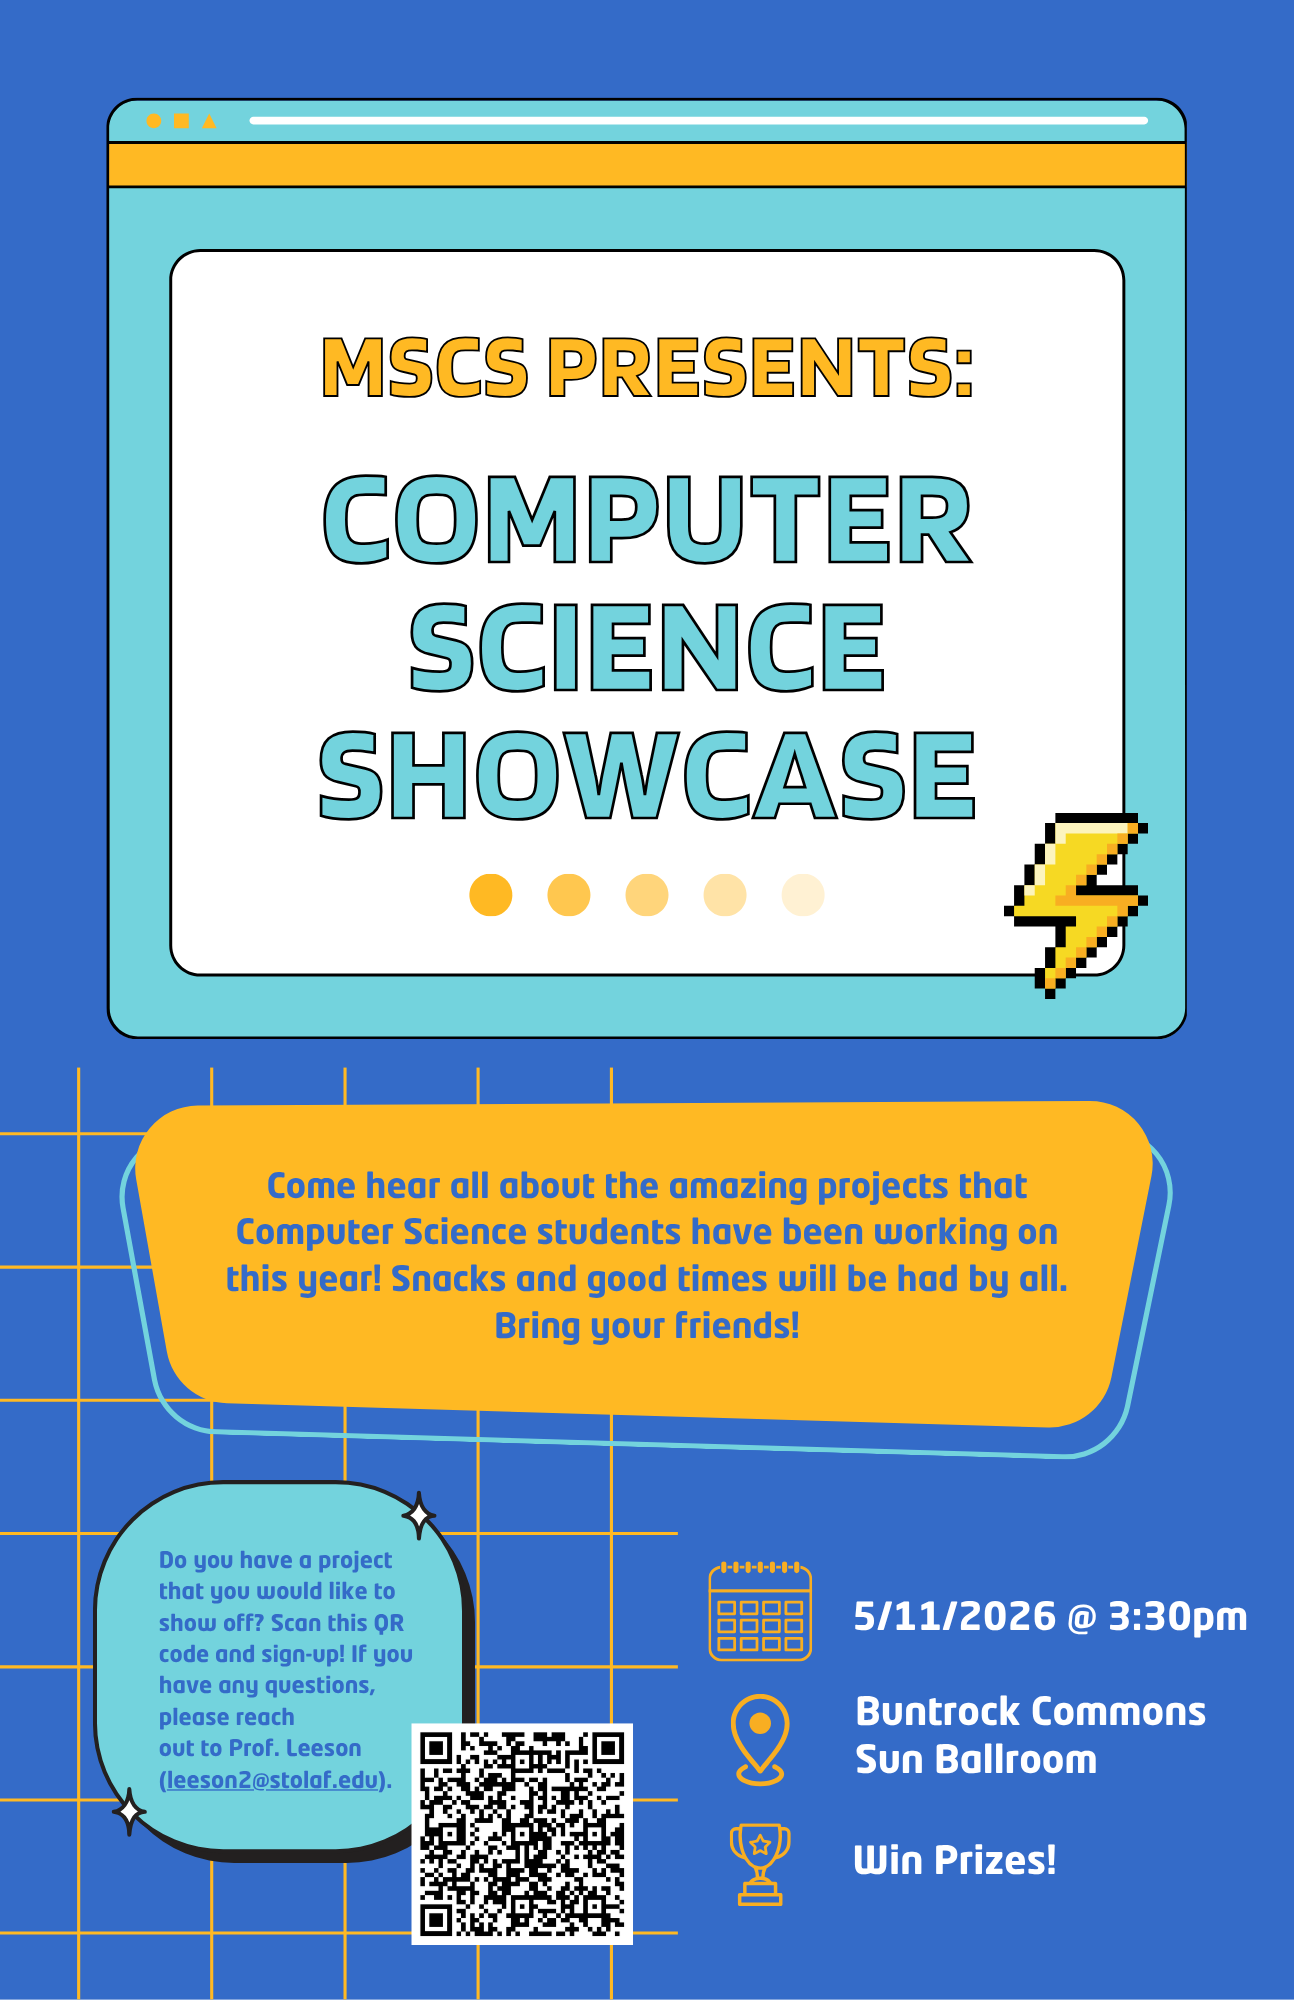
\includegraphics[height=0.95\textheight]{images/Computer Science Showcase (1).png}
\end{center}

\begin{center}
    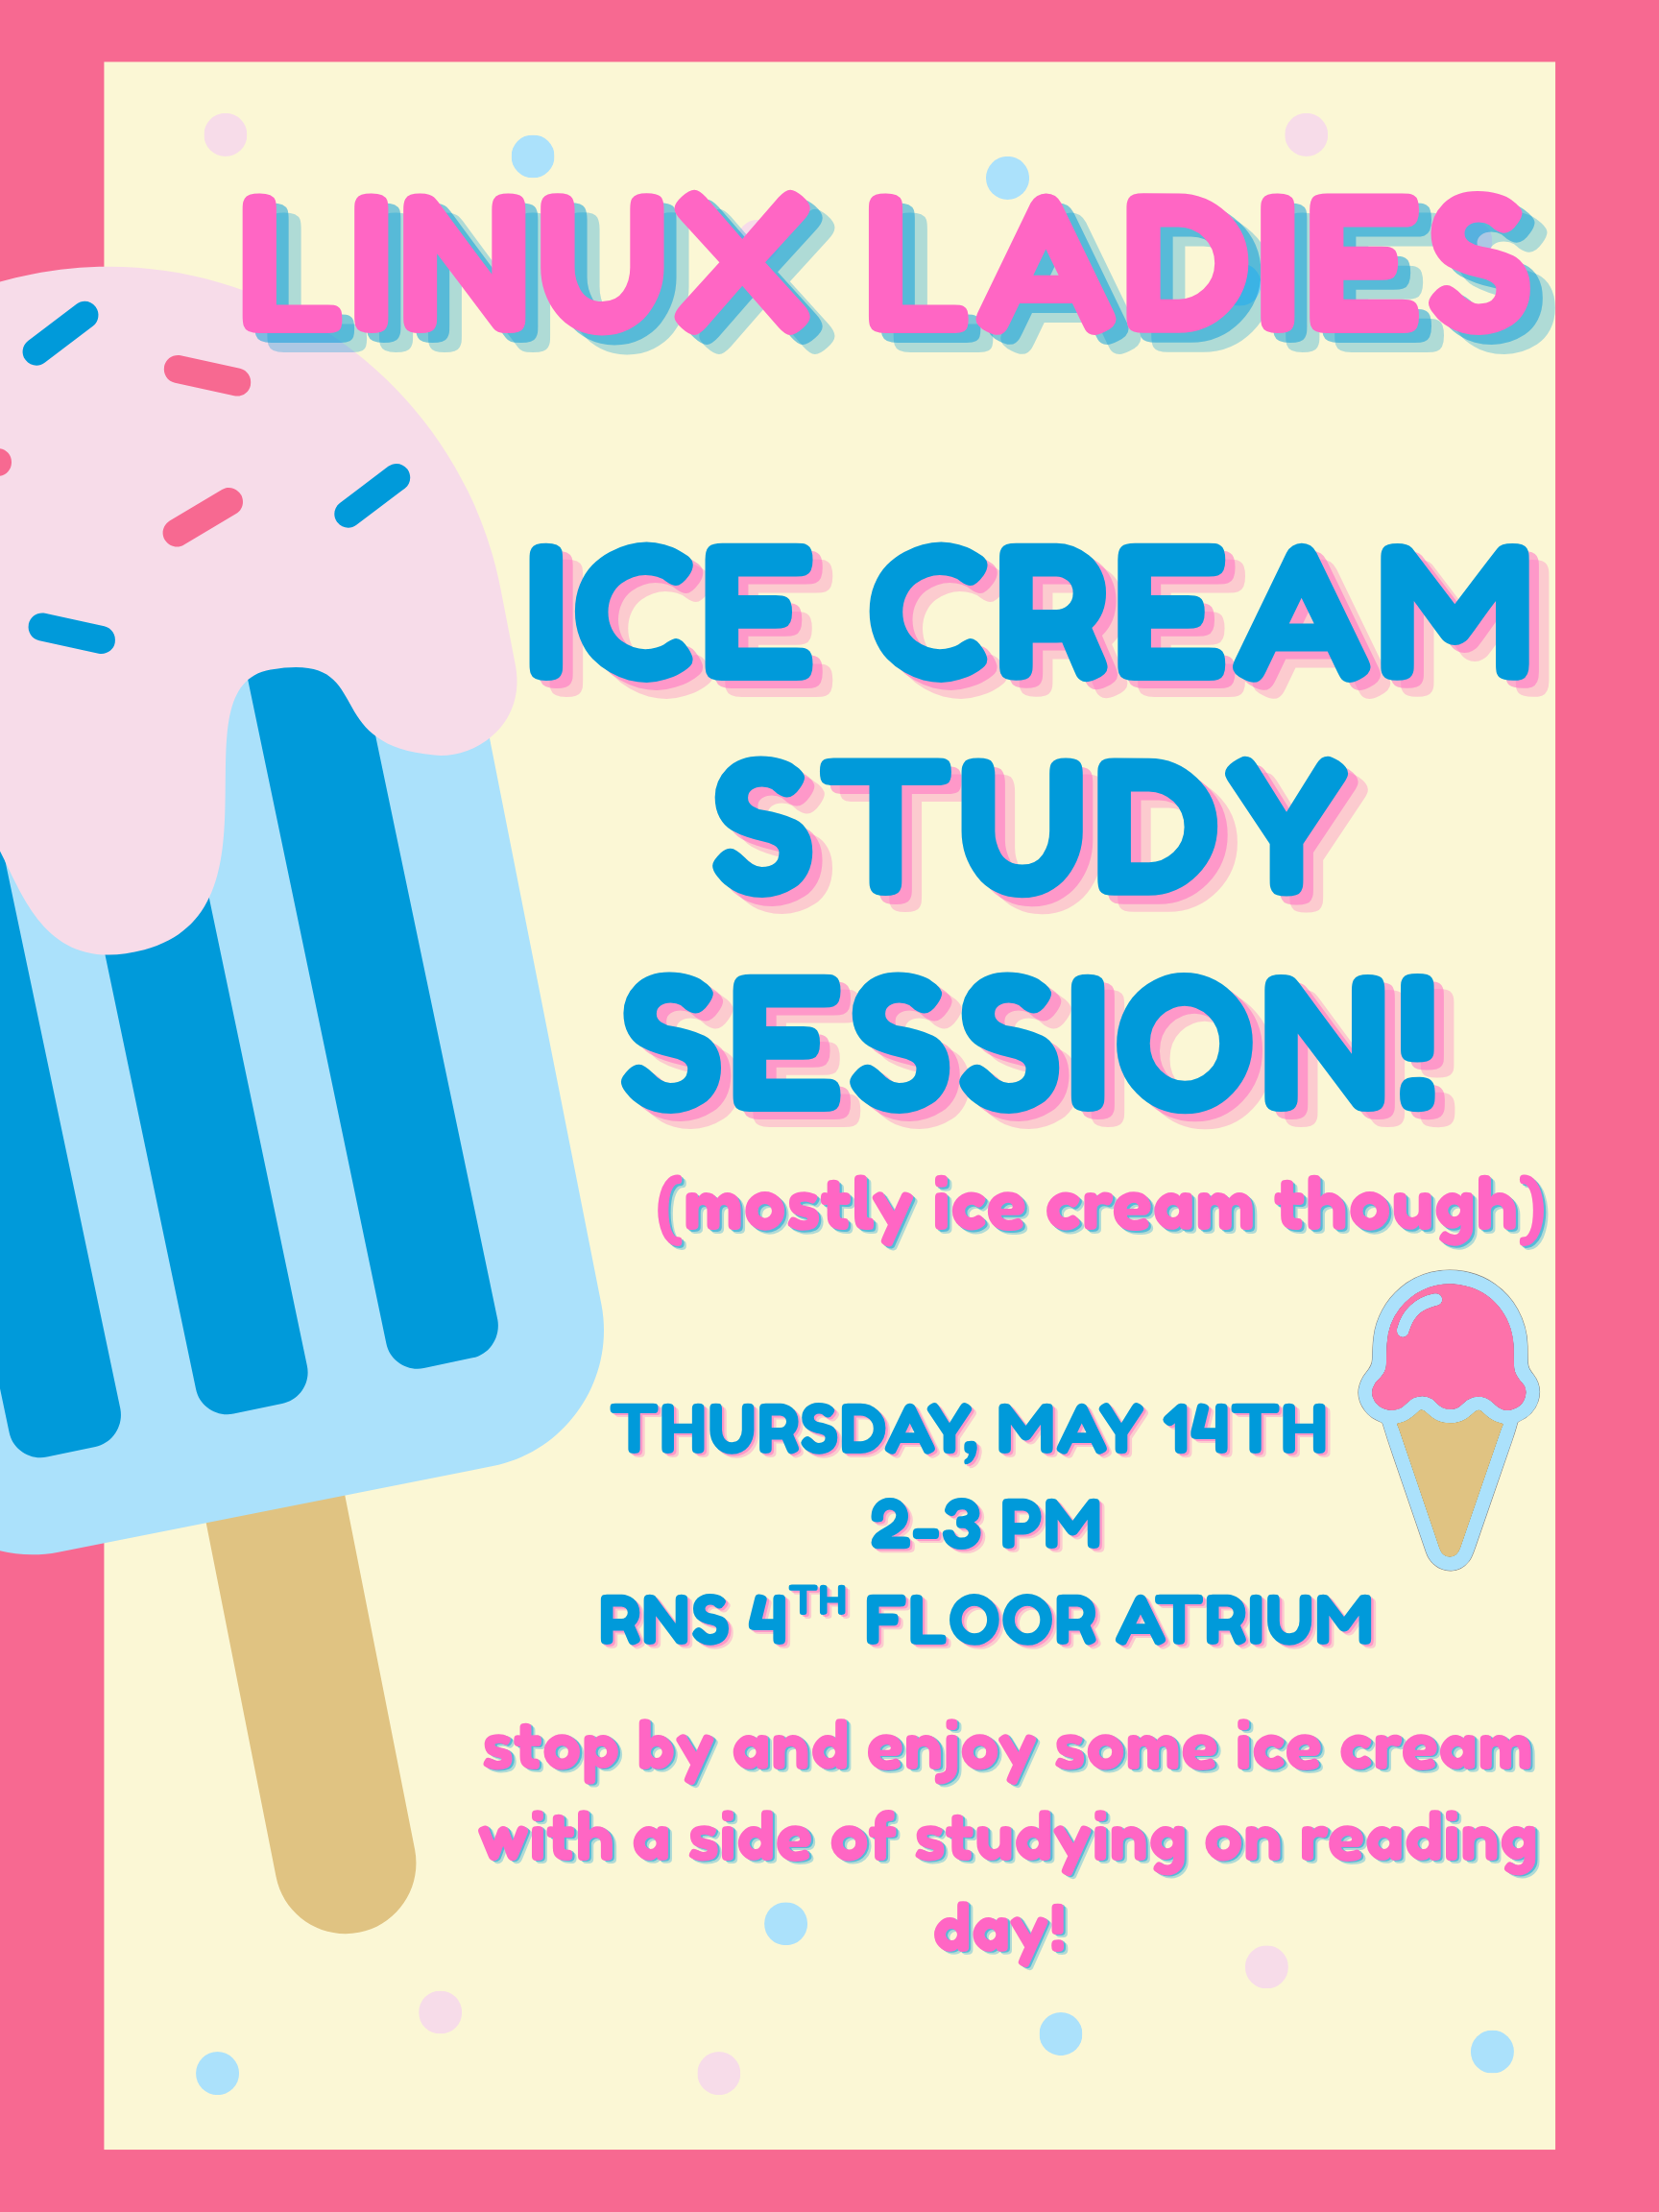
\includegraphics[height=0.95\textheight]{Ice Cream Social-2.png}
\end{center}

\begin{center}
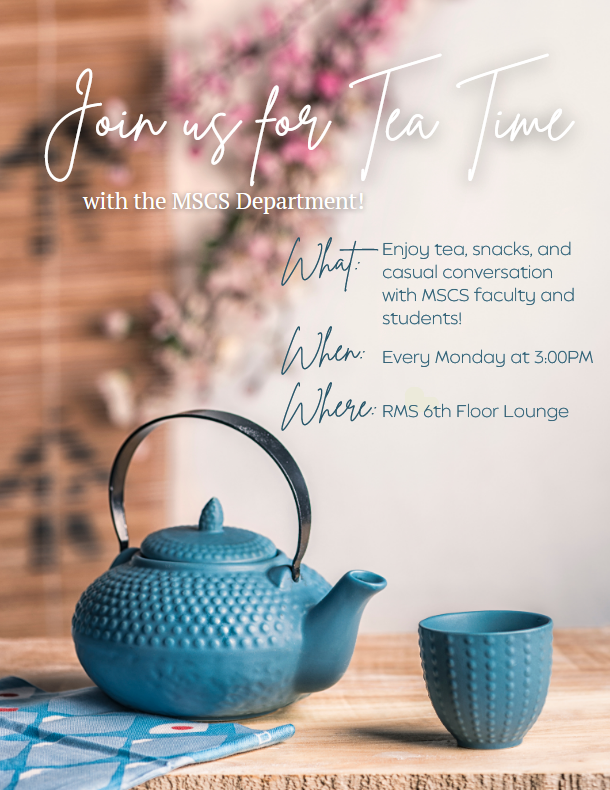
\includegraphics[width=0.9\textwidth]{images/Tea Time Poster.png}
\end{center}

\noindent{To submit an article, event, or anything else for publication in the Mess, email messeditor@stolaf.edu. Visit \href{https://wp.stolaf.edu/mscs/mscs-mess/}{http://wp.stolaf.edu/mscs/mscs-mess/} for a digital archive of previous MSCS Mess issues.}\\
	
\hfill Nima Dahir, Editor
	
\hfill Kyle Salois, Faculty Advisor


 

\end{document}